\documentclass{standalone}
\usepackage{tikz}
\usetikzlibrary{patterns, angles}
\usepackage{circuitikz}

\begin{document}
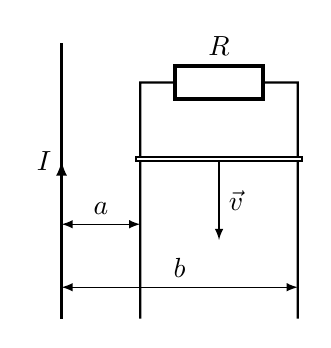
\begin{tikzpicture}[european]
	\draw [thick, arrows={-latex}] (0,0) -- (0,2) node [left] {$I$};
	\draw [thick] (0,1.5) -- (0,3.5);
	\draw [thick] (1,0) -- (1,3) to [R=$R$] (3,3) -- (3,0);
	\draw [thick, fill=white] (0.95, 2) rectangle (3.05,2.05);
	\draw [arrows={-latex}] (2,2)--(2,1) node [midway, right] {$\vec{v}$};
	\draw [arrows={latex-latex}] (0,1.2) -- (1,1.2) node [midway, above] {$a$};
	\draw [arrows={latex-latex}] (0,0.4) -- (3,0.4) node [midway, above] {$b$};
\end{tikzpicture}
\end{document}